
% ==========================================
\section{Controlled experiments}
\label{Synthetic_exp}

With the goal of finding the regime of hyper parameters and optimization techniques where multi-region demixing works best , we start with a series of experiment where we mixed known expression profiles in a controlled way. This allowed us to solve multi-region demixing in a settings where the latent factors are known and used as a ground truth. We first describe how the dataset was created and then characterize how performance depends on the number of samples and the number of latent factors (cell types).

\subsection{Creating the mixture dataset}
We created controlled mixtures from a set of real transcriptome measurements, measured using microarrays from isolated cells. \citet{okaty2011cell} collected 195 cell-type-specific profiles from 64 cell types spanning multiple regions and layers of the mouse brain. These profiles were previously measured after isolating cell using various techniques (FACS, LMD). Although our goal is to use this method on RNA sequencing data which is more quantitative, there is yet no dataset that preformed RNA sequencing of single cell type from multiple brain regions. So to validate our method on controlled set we use microarray data.
 
Specifically, we create known latent factors from expression profiles of the 3 major population of cell types in the brain: neurons, astrocytes and oligodendrocytes, each represented by 14580 genes. Profiles were extracted from 7 brain regions used in \citet{doyle2008}:  cortex layer 5A, cortex layer 5B, cortex layer 6, striatum, cerebellum, brainstem and the spinal cord. For each of these region, we also found the proportions of the three cell types reported in the literature \cite{Herculano2014}. (cortex:  0.7,0.1,0.2 for neuron, astrocytes, oligodendrocytes; cerebellum: 0.5,0.15,0.35, other: 0.65,0.1,0.25). To draw a mixture sample, we drew proportion values $p_{neuron},p_{astro},p_{oligo}$ by adding multiplicative noise to the literature proportions. Each proportion was multiplied by a random value in [0,1] and scaled back to a  sum of 1. Finally, we added multiplicative Gaussian noise to the expression level of all genes, of the form $N(1,\xi^2)$, with noise levels of $\xi=10\%$.

We then used the known mixtures to test the quality of reconstructed profiles as a function of number of samples, noise level, number of factors, and the optimization algorithm. 


\subsection{Evaluation criteria}
We evaluated the quality of a demixing method by computing the fraction of expression variance that it explains. The unexplained (residual) variance is computed as $1-\rho^2$, where $\rho$ is the spearman correlation between the predicted profile and the ground truth profile.

When predicting profile of multiple cell types (like neurons, astrocytes and oligodendrocytes), we first match each the three inferred profiles to the three ground truth profiles, such that the sum of their three spearman correlations is maximized. This little maximization search may introduce a positive bias. To correct for this bias, we compute the following bootstrap baseline. Three expression samples are drawn randomly from the set of samples, the triplet is matched to the ground truth, and its median spearman correlation is computed. This process was repeated 100 times to give a bootstrap estimate. Figure 1(a-c) report these scores using the unexplained variance $1 - spearman$.


prerdicted profiles by computing their %spearman correlation with the true profiles. We then, %matched the best true profiles to the reconstructed %profiles.

%Each time we sampled n noisy samples and reconstructed the %profiles using these samples. The error bars in figure  %represented the sem over 30 repetitions.  

\subsection{Comparing optimization methods for single region NMF}
The NMF optimization problem is non convex, hence different optimization techniques often reach different local minima even when initialized using the same starting points. These performance differences can result from the optimization procedure (MU or ALS) or from stopping conditions and convergence rates. Figure \ref{fig:controlled_exp}(a) compares the performance of 4 optimization algorithms on expression profiles from a single region (cortex layer 5). 

All four methods improve with the number of samples, and saturate near 50 samples. For small number of samples, the block-pivoting and the active-set performed slightly better than other approaches, and almost identical to each other (their graph overlaps). We concluded that active-set ALS is our method of choice.

\subsection{Tuning the strength of pairwise attractive potential}
Next, we applied multi-region demixing (Algorithm 1) to the controlled data mix described above, and tested its accuracy as a function of the global hyperparameter $\lambda$ controlling the strength of attraction among region pairs. Figure 2B shows that in the regime of small sample size, which is relevant to the brain datasets we work with, there is sweet spot where $\lambda=0.1$ outperforms extreme values of $\lambda$. Specifically, both the case of $\lambda=0$ (no sharing, demixing each region individually) and the case of $\lambda \gg0$ (maximum sharing, brain as a single homogeneous region) performed much worse. This suggests that the soft sharing of regio profiles is beneficial in this data.  

As the number of samples increases the benefit of sharing across regions diminishes (Figure \ref{fig:controlled_exp}(b)), and with enough samples per region solving the individual problems performs almost just as well. 

Finally, \ref{fig:controlled_exp}(c) shows the unexplained variance as a function of $\lambda$ for 3 to 5 latent factors (cell types). As the number of types increases, the models are richer and could in theory fit the data better (due to the bias discussed in the evaluation criteria section above). However, this effect does not seem to be significant in this data.  Instead, it seems that the multi-region demixing recovered the three original profiles and some other vectors which helped to lower the overall fit but not the correlation to the original profiles. 
\begin{figure}[!hbt]
   (a) \hspace{120pt}(b) \hspace{120pt}(c) \hspace{190pt}
   \centering
     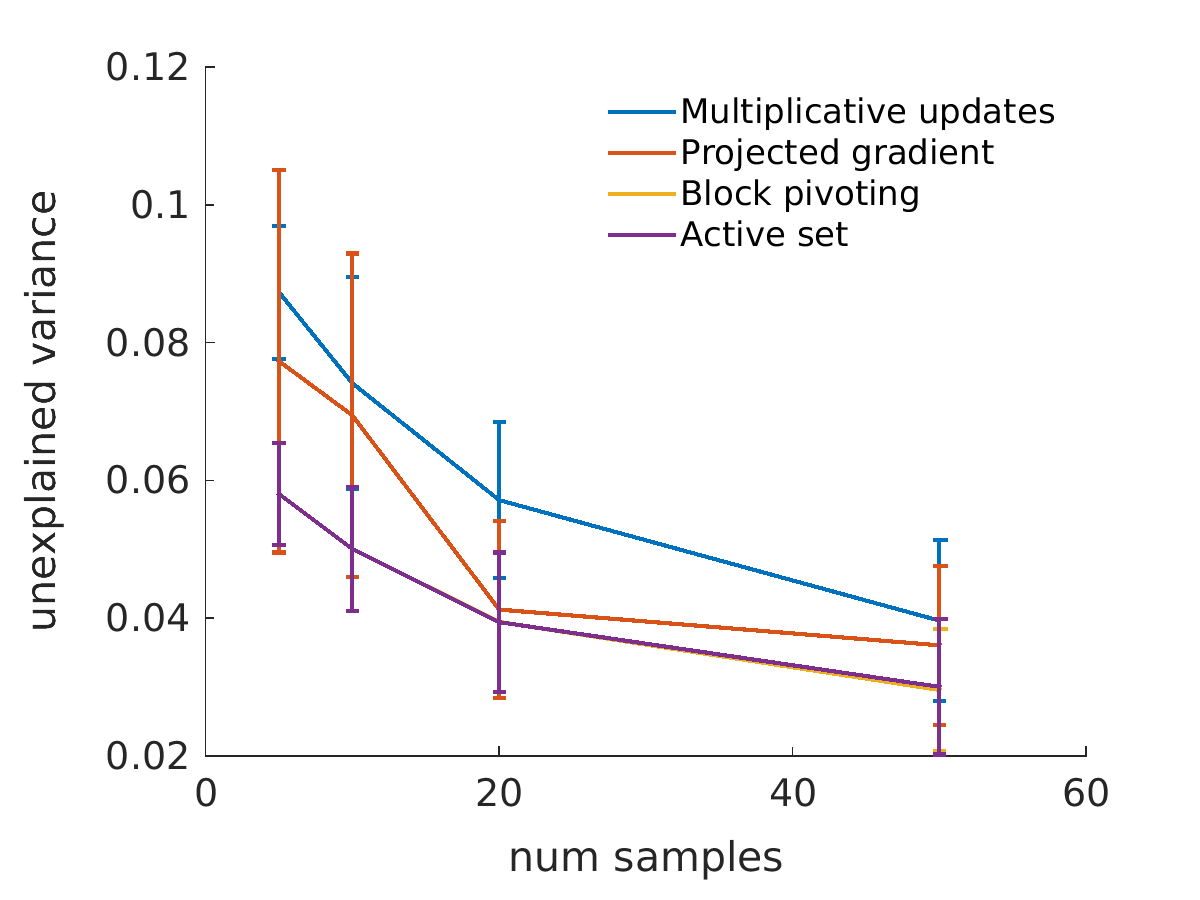
\includegraphics[width=0.32\textwidth]{methods}
     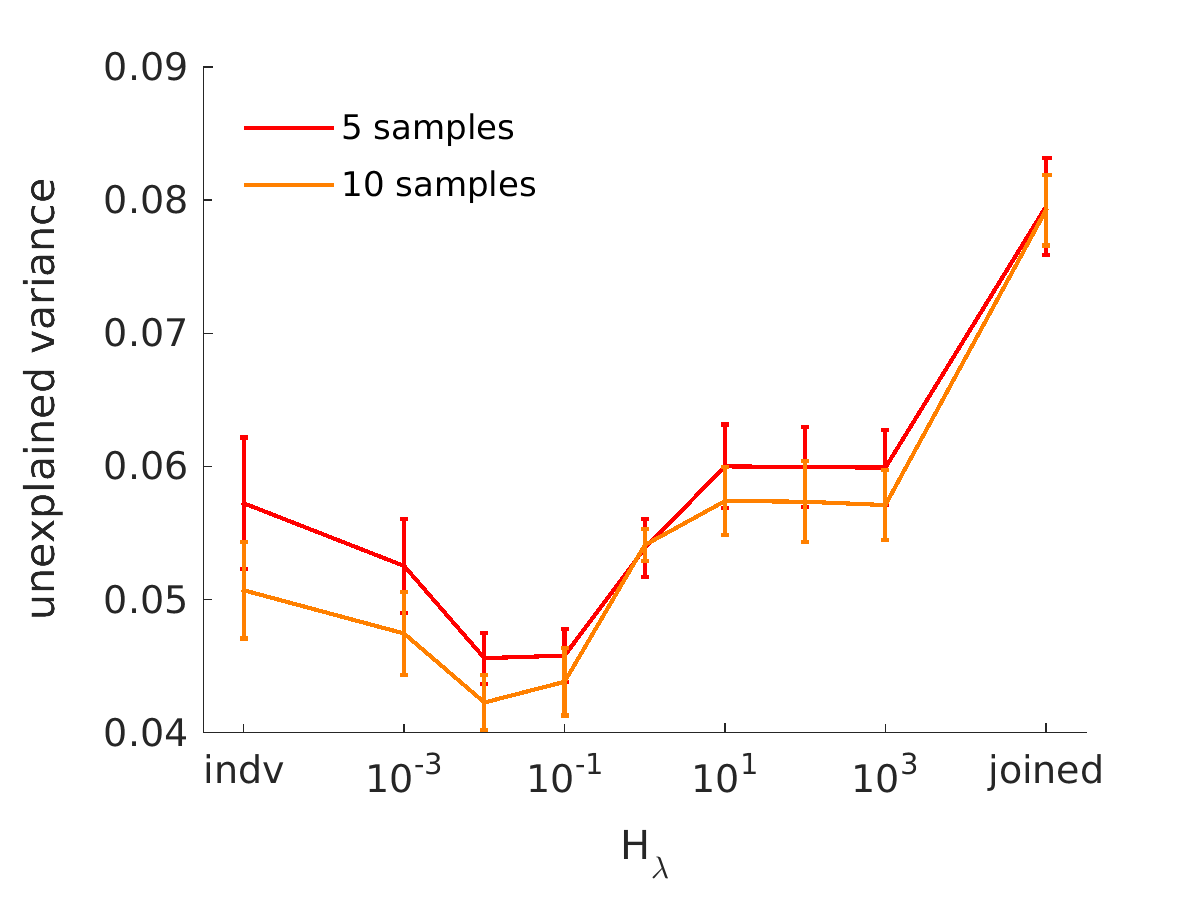
\includegraphics[width=0.32\textwidth]{lambda_samples}
     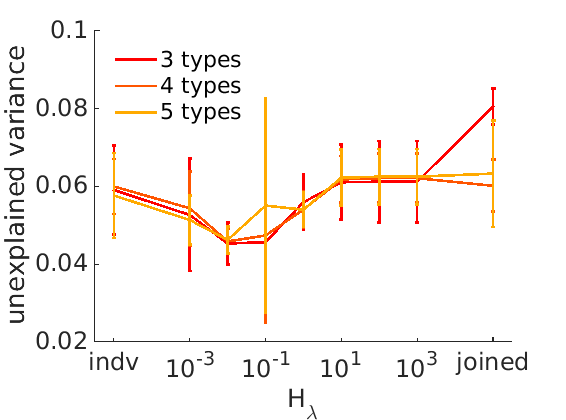
\includegraphics[width=0.32\textwidth]{num_types}
    \caption{Demixing in controlled experiments. 
    {\bf{(a)}}  Within a single region, all optimization methods improve when using more samples. The {\em active set} approach and the {\em block pivoting} outperformed other methods, particularly with few samples. {\bf{(b)}} Soft-sharing of latent factors lead to improved reconstruction in the 7-region settings, particularly with few samples. Results are shown for optimizing with 7 brain regions. {\bf{(c)}} Reconstruction using more cell types then needed does not improve the results.} 
    \label{fig:controlled_exp}
\end{figure}

We found that the use of priors was somewhat fragile. While prior that were taken from the same experiment helped to imporve the score, priors of the same cell type just gathered in different experiments lowered our demixing success. 

% ==========================================
\section{Experiments with postmortem human brain expression}
\label{Human_exp}

We turn to analyze real mixtures collected using RNA-seq measurements from postmortem human brains. We used data from brainspan \cite{brainspan} (\url{http://www.brainspan.org/} and limited analysis to donors older than 17 years, leaving 8 adult human donors. We therefore had eight samples from each brain region. Each expression profile is represented by a vector of 52376 measurements including transcripts counts for coding and non-coding sequences. 

%Collecting human brain measurements is not easy to task since the the tissues has to be extracted not long after the subject death. So while the expression in each tissue can be represented in more details with the advancement of the sequencing tools, the number of samples is still extremely limited. For example, in our dataset there only few dozen samples and each is representation by tens of thousands features.

RNA sequencing is becoming the main way to measure gene expression in tissues, replacing the older microarrays technology. RNA sequencing provides more quantitative measurement since it actually counts the number of RNA transcripts in a tissue, as opposed to the more qualitative microarrays measurements. As such, RNA-seq data is more suitable for demixing since the number of RNAs transcripts grows linearly with the proportion of corresponding cells in the tissue.

To evaluate the quality of demixing, we compare the inferred hidden cell-type specific profiles to transcriptome profiles measured in population of cells sorted by their cell type. At the time we conducted the analysis the cell-type specific RNA-seq data were only available in mouse \cite{barres2014}. We mapped the genes in the human to their orthologs in mouse and computed the spearman correlation between the reconstructed profiles and each of the single cell profiles. Recently such cell-type-specific data was made available for human, which will allow us to perform better validations. 

We determined the strengths of region-to-region relatedness $\phi_{r,s}$ based on the brain-region-ontology described in Figure \ref{fig:bro}. To verify that the human transcriptome measurements agree with this ontology, we first used an agglomerate hierarchical clustering over regions, by clustering expression profiles of these regions collected using microarray data by \cite{kang2011spatio}. The resulting region hierarchy had very string agreement with the brain region ontology, consistent with previous reports that adult expression patterns reflect brain development \cite{zapala2005}. The strengths of region-to-region attractive potentials $\lambda_{r,s}$ was determined as $\lambda \phi_{r,s}$ where $\lambda$ is a hyper parameter controlling the overall weight of edge potentials. 

Figure 3 shows the residual variance computed based on a spearman correlation between the predicted and ground truth profiles, for three cell types and 5 brain regions. The details of the evaluation procedure was explained in section 5.2 above. We selected the 5 brain regions by selecting 3 subcortical regions and 2 cortical regions that were most remote (dorsolateral prefrontal cortex and primary visual cortex).

At the optimal predicted expression profiles, the residual unexplained variance is reduced by 7\% for neurons, 8\% for astrocytes and 5\% in oligodendrocytes, going down to $35\%$ unexplained variance for neurons. To get a scale of these numbers, we computed the correlation between expression profiles of isolated cortical neurons, measured by different labs and avialble through the dataset of \cite{okaty2011cell}. The median spearman correlation across these profiles was ~0.87, or 25\% unexplained variance. It is to beexpected that the correlation with human brain profiles would be even lower. This suggests that reducing the unexplained variance to these levels may be 


% As a comparison, we estimated 


% We compared our results with those of random baseline that was obtained by repeatedly selecting a set of 3 samples as the reconstructed profiles. It should be notated that even single cell experiments that are gathered from the same species in different experiment and from different region is only correlated to the other samples from the same type by 0.877. 
% We notice that for most parts we are able to improve the reconstruction over the baseline. The use of the % regions prior also improves the demixing over the demixing obtained using each brain region individually.



\begin{figure}[!hbt]
    \label{fig:human}
   (a) \hspace{120pt}(b) \hspace{120pt}(c) \hspace{120pt}
   \centering
     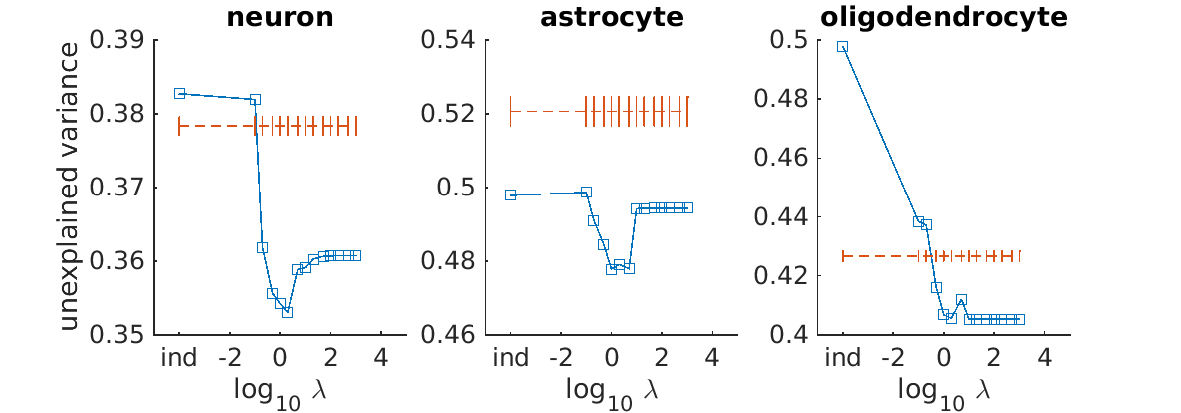
\includegraphics[width=0.99\textwidth]{3panels_var_AMY-CBC-DFC-HIP-V1C.png}
     \caption{Demixing RNA-seq data from 5 human brain regions \cite{brainspan}. Blue curve and squares correspond to the residual variance $(1-\rho^2)$ as a function of the strength of attractive region-to-region potentials $\lambda$. Red dashed line corresponds to a best-matched samples baseline (Sec 5.2).}
    
\end{figure}


% [Add in the human experiment section We first verified that the brain regions in our data agree with the dev ontology: we clustered the brain regions in a hierarchical way and compared the resulting hierarchy to the dev ontology. We obtained very strong agreement …]. 
